\documentclass[tikz,border=8pt]{standalone}
% Shared look for every TikZ diagram. Load with % Shared look for every TikZ diagram. Load with % Shared look for every TikZ diagram. Load with \input{../../tools/tikz-style.tex}
\usepackage[T1]{fontenc}
\usepackage{lmodern}
\renewcommand{\sfdefault}{lmr}  % diagrams use the same serif as the text
\usetikzlibrary{arrows.meta, positioning, shapes.geometric, calc, fit, backgrounds}
\definecolor{cblue}{HTML}{4C78A8}
\definecolor{corange}{HTML}{F58518}
\definecolor{cgreen}{HTML}{54A24B}
\definecolor{cred}{HTML}{E45756}
\definecolor{cpurple}{HTML}{B279A2}
\definecolor{cgrey}{HTML}{6B6B6B}
\tikzset{
  every picture/.style={font=\sffamily, line width=1.2pt},
  box/.style={draw=#1, fill=#1!12, rounded corners=4pt, align=center, inner sep=7pt, minimum height=1.1cm},
  box/.default=cgrey,
  arrow/.style={-{Stealth[length=3mm]}, draw=cgrey, line width=1.4pt},
  title/.style={font=\sffamily\bfseries\Large},
  note/.style={font=\sffamily\small, text=cgrey, align=center},
}
\AtBeginDocument{\hyphenpenalty=10000 \exhyphenpenalty=10000}

\usepackage[T1]{fontenc}
\usepackage{lmodern}
\renewcommand{\sfdefault}{lmr}  % diagrams use the same serif as the text
\usetikzlibrary{arrows.meta, positioning, shapes.geometric, calc, fit, backgrounds}
\definecolor{cblue}{HTML}{4C78A8}
\definecolor{corange}{HTML}{F58518}
\definecolor{cgreen}{HTML}{54A24B}
\definecolor{cred}{HTML}{E45756}
\definecolor{cpurple}{HTML}{B279A2}
\definecolor{cgrey}{HTML}{6B6B6B}
\tikzset{
  every picture/.style={font=\sffamily, line width=1.2pt},
  box/.style={draw=#1, fill=#1!12, rounded corners=4pt, align=center, inner sep=7pt, minimum height=1.1cm},
  box/.default=cgrey,
  arrow/.style={-{Stealth[length=3mm]}, draw=cgrey, line width=1.4pt},
  title/.style={font=\sffamily\bfseries\Large},
  note/.style={font=\sffamily\small, text=cgrey, align=center},
}
\AtBeginDocument{\hyphenpenalty=10000 \exhyphenpenalty=10000}

\usepackage[T1]{fontenc}
\usepackage{lmodern}
\renewcommand{\sfdefault}{lmr}  % diagrams use the same serif as the text
\usetikzlibrary{arrows.meta, positioning, shapes.geometric, calc, fit, backgrounds}
\definecolor{cblue}{HTML}{4C78A8}
\definecolor{corange}{HTML}{F58518}
\definecolor{cgreen}{HTML}{54A24B}
\definecolor{cred}{HTML}{E45756}
\definecolor{cpurple}{HTML}{B279A2}
\definecolor{cgrey}{HTML}{6B6B6B}
\tikzset{
  every picture/.style={font=\sffamily, line width=1.2pt},
  box/.style={draw=#1, fill=#1!12, rounded corners=4pt, align=center, inner sep=7pt, minimum height=1.1cm},
  box/.default=cgrey,
  arrow/.style={-{Stealth[length=3mm]}, draw=cgrey, line width=1.4pt},
  title/.style={font=\sffamily\bfseries\Large},
  note/.style={font=\sffamily\small, text=cgrey, align=center},
}
\AtBeginDocument{\hyphenpenalty=10000 \exhyphenpenalty=10000}

\begin{document}
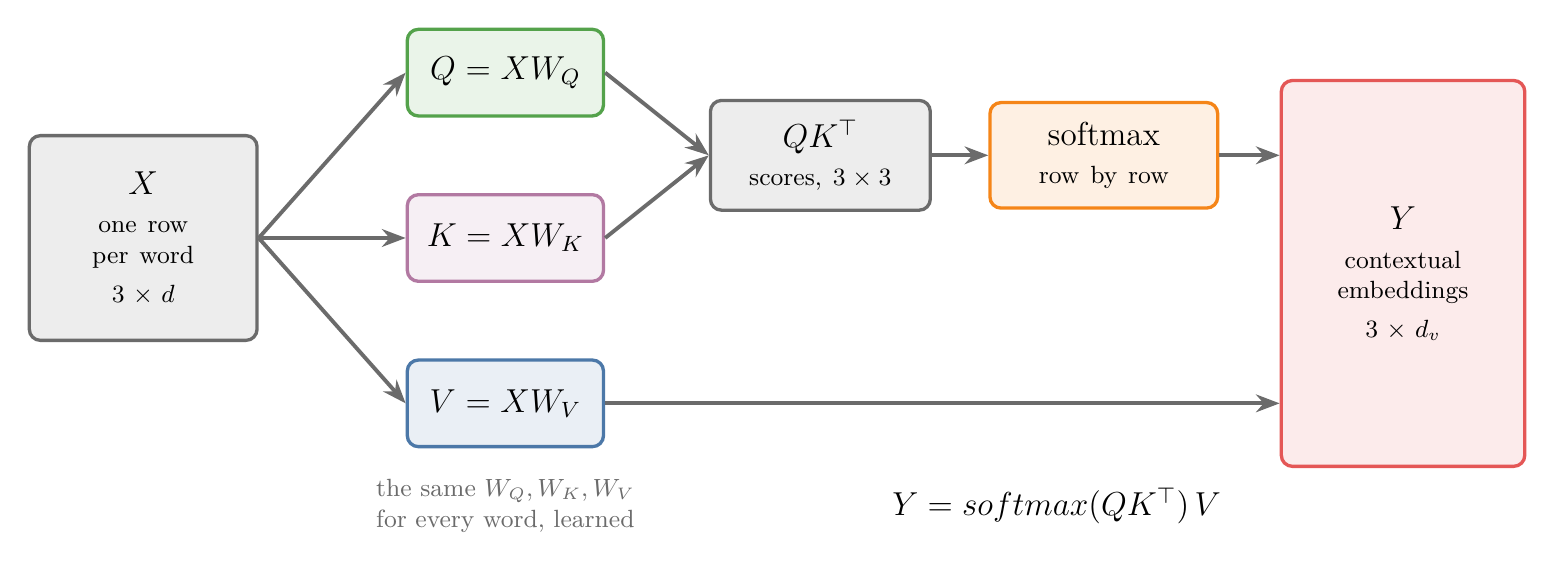
\begin{tikzpicture}[every node/.append style={font=\sffamily\large}]
  \node[box=cgrey, text width=2.4cm, minimum height=2.6cm] (X) at (0,0) {$X$\\[3pt]\small one row per word\\$3 \times d$};
  \node[box=cgreen, text width=2.0cm] (Q) at (4.6,2.1) {$Q = XW_Q$};
  \node[box=cpurple, text width=2.0cm] (K) at (4.6,0) {$K = XW_K$};
  \node[box=cblue, text width=2.0cm] (V) at (4.6,-2.1) {$V = XW_V$};
  \foreach \m in {Q,K,V} \draw[arrow] (X.east) -- (\m.west);
  \node[box=cgrey, text width=2.3cm] (S) at (8.6,1.05) {$QK^{\top}$\\\small scores, $3 \times 3$};
  \draw[arrow] (Q.east) -- (S.west); \draw[arrow] (K.east) -- (S.west);
  \node[box=corange, text width=2.4cm] (W) at (12.2,1.05) {softmax\\\small row by row};
  \draw[arrow] (S) -- (W);
  \node[box=cred, text width=2.6cm, minimum height=4.9cm] (Y) at (16.0,-0.45) {$Y$\\[3pt]\small contextual\\embeddings\\$3 \times d_v$};
  \draw[arrow] (W.east) -- (Y.west |- W.east);
  \draw[arrow] (V.east) -- (Y.west |- V.east);
  \node[note, text width=4.2cm] at (4.6,-3.4) {the same $W_Q, W_K, W_V$\\for every word, learned};
  \node[font=\sffamily\bfseries\large] at (11.6,-3.4) {$Y = \text{softmax}(QK^{\top})\,V$};
\end{tikzpicture}
\end{document}
